\documentclass{beamer}
\usetheme{Boadilla}

\title{Digital Forensics}
\subtitle{File System Forensics Masterclass}
\author{Fraser Brown}
\institute{Heriot-Watt University}
\date{\today}

\graphicspath{{../figures/}}

\begin{document}

\begin{frame}
\titlepage
\end{frame}

\begin{frame}[shrink]
\section{Overview}
\frametitle{Outline}
\tableofcontents
\end{frame}

\begin{frame}
	\frametitle{What is Digital Forensics}
	\section{What is Digital Forensics?}
%	\begin{itemize}
%		\item Digital forensics is a pulls from both cyber security and forensic science fields.
%	\end{itemize}
	\begin{block}{Digital Forensics:}
		``Computer [Digital] Forensics is the practice of determining the past actions that have taken place on a computer system using forensic techniques and understanding artefacts.'' - David Cowen
	\end{block}
		
	\begin{block}{Artefact:}
		``An Artefact is a reproducible file, setting or system change that occurs every time an application or operating system performs a specific action'' - David Cowen
	\end{block}

	The artefacts we will be dealing with in the lab are files and file systems.
\end{frame}

\begin{frame}[allowframebreaks]
	\frametitle{Why File System Analysis?}
	\section{Why File System Analysis?}
	\begin{itemize}
		\item There are many different forms of digital forensic analysis:
			\begin{itemize}
				\item Network Analysis,
				\item Live memory (RAM) Analysis, 
				\item File system analysis, 
				\item Database Analysis,
				\item Application/OS Analysis
			\end{itemize}
			\item File system analysis allows:
			\begin{itemize}
				\item Introduction to a new field using a common ground
				\item Insight into how OS files relate to memory and what creation and deletion features actual do
			\end{itemize}
	\end{itemize}
	\begin{figure}
		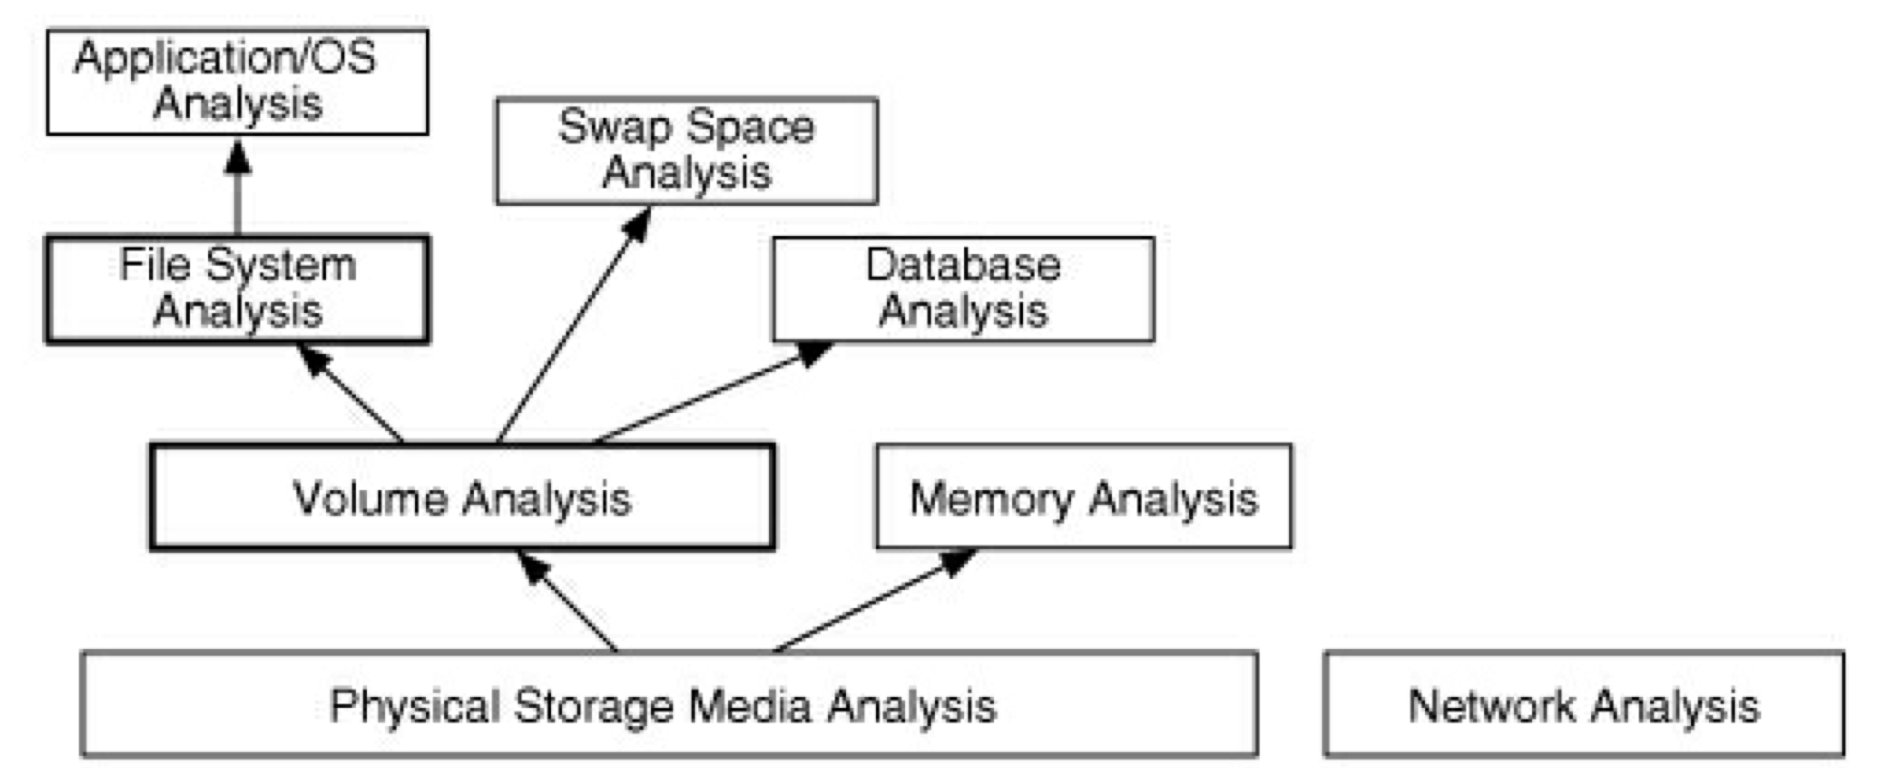
\includegraphics[scale=0.3]{digital-data-analysis-layers-BrianCarrier}
		\caption{Layers of Analysis}
	\end{figure}
\end{frame}

\begin{frame}
	\frametitle{Forensic Process}
	\section{Forensic Process}
	Digital forensics results can be used in a court of law therefore accuracy, integrity and an unbiased approach towards evidence is required.\\
	As a result similar approaches to evidence handling and procedure from traditional forms of forensics are utilised.   
	\begin{block}{Scientific Method}
		Defining a hypothesis based on evidence then proceeding search for evidence which disproves our hypothesis.
	\end{block}
	\begin{block}{Digital Forensic Investigation}
	``A digital forensic investigation is a process that uses science
     and technology to analyse digital objects and that develops and
     tests theories, which can be entered into a court of law, to
     answer questions about events that occurred. In other words, a
     digital forensic investigation is a more restricted form of
     digital investigation.'' - Brian Carrier
	\end{block}
\end{frame}

\begin{frame}[fragile]
	\frametitle{Digital Crime Scene Investigation Process Overview}
	\subsection{Digital Crime Scene Investigation Process Overview}
	There are three major areas in digital crime scene investigations:
	\begin{itemize}
		\item System Preservation
		\item Evidence Searching
		\item Event Reconstruction
	\end{itemize}
	\begin{figure}
		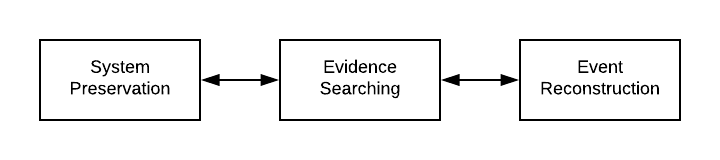
\includegraphics[scale=1]{df-guidelines}
		\caption{Diagram of Digital Forensics Investigation Phases}
		\label{fig:df-guidelines}
	\end{figure}
\end{frame}

\begin{frame}
	\frametitle{PICL Guidelines}
	\subsection{PICL Guidelines}
	While each forensic investigator/team may have their own procedures and work flow the PICL guidelines below provide a good staring structure:
	\begin{itemize}
		\item Preservation:	 Preservation of the system being investigated.
		\item Isolation:	 Keeping analysis environment is separate from both the suspect data and the outside world.
		\item Correlation:	 Correlate data with other independent sources. Reduces risk of forged data.
		\item Logging:	 Log/document your actions. This helps identify what searches you have not yet conducted and what your results were.
	\end{itemize}
\end{frame}

\begin{frame}
	\frametitle{Analysis Types}
	\subsection{Analysis Types}
	\begin{block}{Live Analysis:}
		``A live analysis occurs when you use the operating system or other resources of the system being investigated to find evidence.'' - Brian Carrier
	\end{block}

	\begin{block}{Dead Analysis:}
		``A dead analysis occurs when you are running trusted applications in a trusted operating system to find evidence.'' - Brian Carrier
	\end{block}
\end{frame}

\begin{frame}
	\frametitle{Evidence Acquisition/Imaging}
	\section{Evidence Acquisition/Imaging}
	\begin{itemize}
		\item In order to perform analysis on digital artefacts a forensic duplicate of the media must be created.
		\item Forensic Duplicates are \emph{bit-for-bit} copies of the original disk and can encompass the full disk or a single partition. 
		\item This process is known as imaging or acquisition.
		\item Contents of a disk are always changing therefore \emph{Write Blockers} are used to preserve the disk state.
		\item Hash functions such as SHA-256, SHA-1, MD5 are used to verify the image against the original artefact.
	\end{itemize}
\end{frame}

\begin{frame}
	\frametitle{Write Blockers}
	\subsection{Write Blockers}
	\begin{block}{Write Blockers}
			Are hardware or software devices that allow gathering of information without damaging the disk contents by blocking write commands but allowing read commands.
	\end{block}
	\begin{itemize}
		\item Write Blockers are customisable:
			\begin{itemize}
				\item Blocking of all or specific commands.
				\item Can control the read and write speed.
			\end{itemize}
		\item Write Blockers come in two forms:
			\begin{itemize}
				\item \emph{Native}: Same interface for input and output e.g. IDE-to-IDE
				\item \emph{Tailgate}: uses different interfaces for input and output e.g. firewire/USB-to-SATA
			\end{itemize}
		\end{itemize}
\end{frame}

\begin{frame}
	\frametitle{Imaging Challenges with Solid State Drives (SSD)}
	\subsection{Imaging Challenges}
	While an SSD can be imaged with the same tools as a traditional hard disk drive (HDD), there are technology specific issues that cause problems for forensic investigators.
	\begin{itemize}
		\item \emph{Program-Erase cycles}
			\begin{itemize}
				\item Sequence of events that result in data being written to a solid state flash memory cell, then erased and rewritten (e.g flash memory USB sticks). 
				\item These P/E cycles result in a small amount of physical damage to the medium, which can result in bad sectors.
			\end{itemize}
		\item \emph{Wear Levelling}
			\begin{itemize}
				\item prolongs the life of solid state/flash memory
				\item Distributes rewrites evenly across the medium, so no single block dies prematurely.
			\end{itemize}
		\item These two technologies due to the evolution of memory results in unallocated space being overwritten earlier than it would on a HDD. This could overwrite valuable hidden information by accident
	\end{itemize}
\end{frame}

\begin{frame}
	\frametitle{Image Types}
	\subsection{Image Types}
	\begin{itemize}
		\item Raw Format (\texttt{.dd} \texttt{.raw} \texttt{.img})
		\begin{itemize}
			\item only contain data from the original artifact
			\item meta data is no included however can be generated into a separate file by tools.
			\item Tools: \texttt{dd}, \texttt{dcfldd}, \texttt{dd\_rescue}, \texttt{rdd}, \texttt{df3dd}, \texttt{guymager}
		\end{itemize}
		\item EnCase Evidence Format (Expert Witness \texttt{.E01})
		\begin{itemize}
			\item Expert Witness images use headers and footers to hold metadata about the image.
			\item metatdata can include: drive type, source disk OS, timestamps, hashes, CRCs over blocks.
		\end{itemize}
	\end{itemize}
\end{frame}

\begin{frame}
	\frametitle{Memory}
	\section{Hard Disk Technology}
		\subsection{Memory Types} %HDD SSD NAND-Flash
		\subsection{Forensics Memory Challenges}
\end{frame}

\begin{frame}
	\frametitle{File System}
	\section{File Systems}
		\subsection{File System Types} %ntfs, fat etc.
\end{frame}

\begin{frame}
	\frametitle{Acquisition and Analysis Tools}
	\section{The Sleuth Kit (TSK)}
		\subsection{TSK Layers}
\end{frame}

\begin{frame}
	\section{Research}
	\frametitle{Digital Forensic Research}
\end{frame}

\begin{frame}
	\section{Additional Resources}
	\frametitle{Additional Resources}
	
\end{frame}

\begin{frame}
	\section{Careers}
	\frametitle{Careers}
	
\end{frame}

\end{document} % End Document